\documentclass{article}
\usepackage{tikz}
\usepackage{listings}

\lstset{frame=tb,language=C++,aboveskip=3mm,belowskip=3mm,showstringspaces=false,columns=flexible,tabsize=3}

\def\checkmark{\tikz\fill[scale=0.4](0,.35) -- (.25,0) -- (1,.7) -- (.25,.15) -- cycle;} 

\title{CS 194 Assignment 1}
\author{Nikhil Unni}
\date{Fall 2015}

\usepackage{natbib}
\usepackage{graphicx}

\begin{document}

\maketitle

\section{Measuring Execution Time}

\begin{table}[!htbp]
\centering
\begin{tabular}{|c|c|c|c|}
 \hline
 O2 Enabled & Printing & Hardcoded number & Number of Ticks\\
 \hline
 \checkmark & \checkmark & \checkmark & 90,646 \\
 \hline
 X & \checkmark & \checkmark & 134,656 \\
 \hline
 \checkmark & X & \checkmark & 1,026\\
 \hline
 X & X & \checkmark & 77,027\\
 \hline
 \checkmark & X & X & 11,584\\
 \hline
 X & X & X & 102,817\\
 \hline
 X & \checkmark & X & 164,476\\
 \hline
 \checkmark & \checkmark & X & 75,250\\
 \hline
\end{tabular}
\caption{Tick Timings for Repeated Addition}
\label{tab:my_label}
\end{table}

\textbf{Explain the discrepancy in timings. (2 points)}

The O2 optimization removes unnecessary instructions (along with other optimizations, like using registers), which is why when its coupled with the ``no printing" option, leads to the fastest execution times, because it can cut out the for loop completely, since it doesn't contribute to the output. The hardcoded number just adds additional time since there is necessary stdin and an O(n) conversion of string to int.\\\\

\textbf{Which configuration is the most accurate way of timing the computation of the sum? (2 points)}

With O2 disabled, printing disabled, and the number hardcoded in. This is because the atoi conversion and stdout printing are not included in the time, but the compiler won't remove the computation completely either.\\\\

\textbf{How does atoi(argv[1]) work? (2 points)}

argv[1] refers to the first argument, a string, supplied by the caller of the program (where argv[0] is the program name itself). atoi() converts a string to an int (``100'' $\rightarrow 100$, for example) by converting each char to an int, and multiplying by some $10^n$.

\section{Measuring Memory Latency}
\textbf{Explain how this pointer chasing benchmark measures the time between requesting and obtaining a value from memory (2 points)}

Because the path traveling indices is randomized, ideally we have an equal mix of cache hits and misses when trying to access the next array index, making us truly measure the time to obtain a value from memory.\\\\

\textbf{How many bytes in memory is an int array of length N on your machine? (1 point)}

4N\\\\

\textbf{Generate a plot of size in bytes of array vs. average number of cycles to execute a step (32 points).}\\
\begin{figure}[!htbp]
  \caption{Int Array Size vs. Average Number of Cycles}
  \centering
    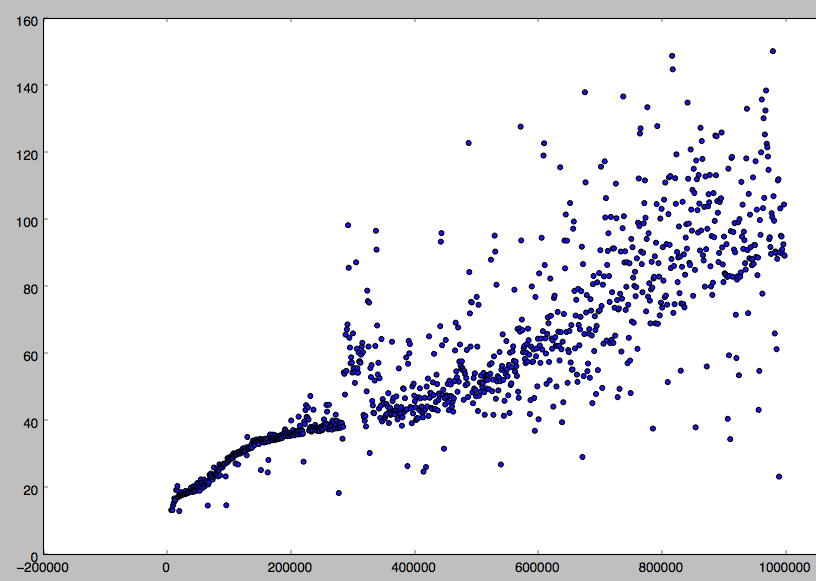
\includegraphics[width=1\textwidth]{screen1}
\end{figure}\\
As a quick note, the x-axis is measuring the array size, rather than size in bytes, so the range is [8000,1000000].\\\\

\textbf{Discuss the shape of the curve (4 points)}

The point where the spread of the points goes crazy is around 1.2MB (or len(array) = 280,000), which is when the computation blew the cache size. From there, you can sort of see a trend going forward, but the points are more normally distributed around the general trend. The reason for the crazy spread is because you can get very small cycles if you're lucky -- for example if A[0] = 2, and A[2] = 0; Worst case, it's a full N-long cycle. When everything could fit on the cache, once you've completed a cycle, every memory access was much faster thereafter.\\\\

\textbf{Do modern out-of-order processors affect our benchmark? (2 points)}

No, it does not, since the processor cannot move ahead, since it cannot ``guess" what the future value will be. Every instruction is constraint by the immediately previous instruction, and that chain cannot be broken anywhere for parallelization.\\\\

\textbf{BONUS (16 points)}

\begin{lstlisting}
int uniqueValues(int *A) {
  int out = 1;
  int fastWalker = A[0], slowWalker = A[A[0]];
  while(slowWalker != fastWalker) {
    slowWalker = A[slowWalker];
    fastWalker = A[A[fastWalker]];
    out++;
  }
  return out;
}
\end{lstlisting}

Essentially, the randomized array is just a linked-list (where the next value is the value at the current index) with a cycle, and we need to determine the cycle size. So we just have a slow walker, which moves traverses the list one at a time, and a fast walker that traverses the list two at a time, and the two are guaranteed to meet at 0, regardless of whether it's even or odd. If the cycle length is even, the fast runner will be at 0 when the slow runner is halfway and when its finally reached zero, where they'll meet. If the cycle length is odd, then the runner will run ``past" 0 twice, the second time, it finally reaching 0, since an odd number times 2 becomes even. Since it's moving twice as fast as the slow runner and takes twice as many cycles to hit 0, the slow and fast runners will yet again meet at 0.

\section{Measuring Memory Bandwidth}

\textbf{Plot the relationships between the average bandwidth and the total size of the array (24 points)}
\begin{figure}[!htbp]
  \caption{my\_memcpy}
  \centering
    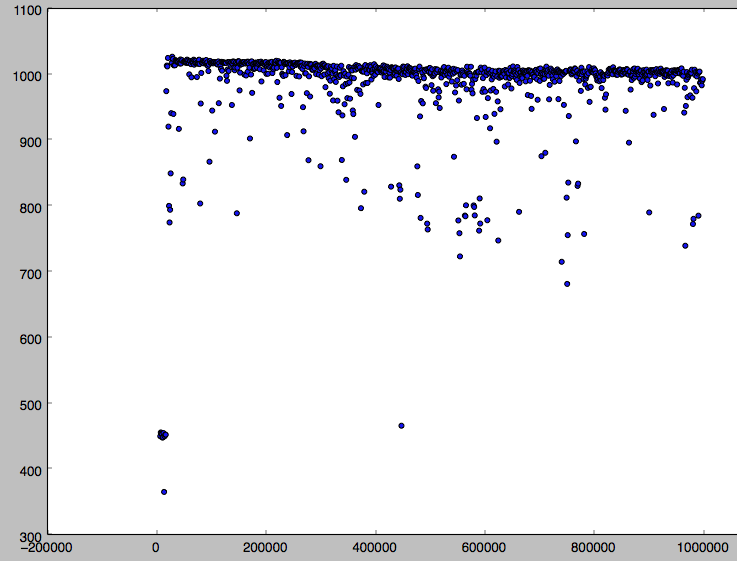
\includegraphics[width=0.75\textwidth]{my_memcpy}
\end{figure}\\

\begin{figure}[!htbp]
  \caption{simd\_memcpy}
  \centering
    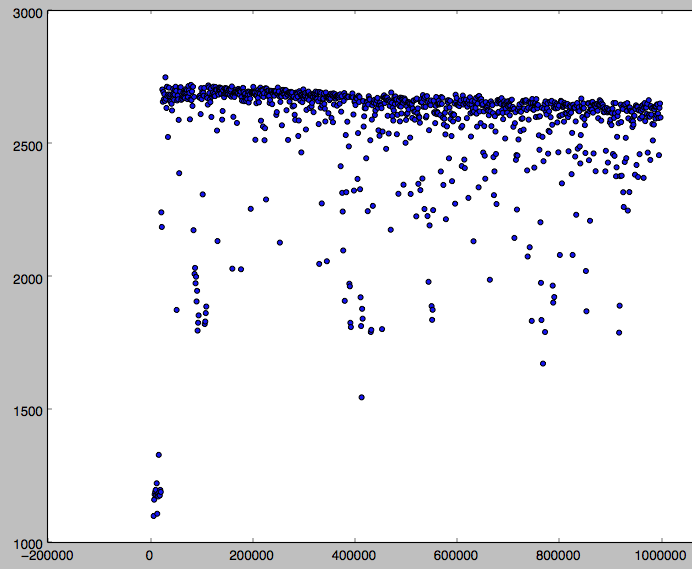
\includegraphics[width=0.75\textwidth]{simd_memcpy}
\end{figure}

\begin{figure}[!htbp]
  \caption{simd\_memcpy\_cache}
  \centering
    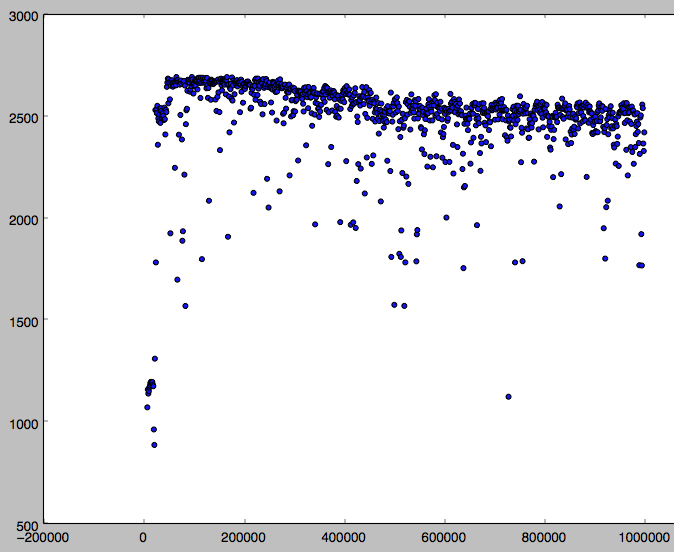
\includegraphics[width=0.75\textwidth]{simd_memcpy_cache}
\end{figure}

\textbf{Discuss the shape of the curve (4 points).}

The three curves generally look the same, except that simd\_memcpy\_cache seems to decrease in bandwidth as the array size increases slightly more than the other two copy methods. There are no meaningful inflection points that I can see in any of the graphs. However, both simd\_memcpy and simd\_memcpy\_cache perform about 2.7x better than my naive my\_copy, that copies over each byte one by one.\\\\

\textbf{Explain why it's necessary to ``warm up the cache" (2 points)}

By copying over the array a few times, we add each of the elements from the src to our cache, so that our copy method has mostly cache hits when it's trying to find values in memory. This will speed up the copy process.\\\\

\textbf{Explain why an inefficient array copying procedure would yield an inaccurate measure of maximum bandwidth}

Because the procedure is inefficient, we're not truly measuring the bandwidth when all resources are used to do the operation. Instead, we get something slower that's not the fastest \textit{possible}.\\\\

\textbf{Find all the different SSE intrinsic calls (6 points)}

\_mm\_prefetch(p, \_MM\_HINT\_NTA) : Prefetches line of data from memory at some address with ``non-temporal allignment," which just suggests that we're not going to go back to that place in memory any time soon, so no need to expect we will.\\

\_mm\_load\_si128 : Loads 128 bit value\\

\_mm\_stream\_si128 : Load 128 bit value, and don't go through cache. Just retrieves value.\\

\_mm\_store\_si128 : Store 128 bit value in memory.

\section{Matrix Multiply}

\textbf{Produce a table recording the Flops and IPC of each matrix multiply}
\begin{table}[!htbp]
\centering
\begin{tabular}{c|c|c|}
 & Flops (GFlops) & IPC (Instr/Cycle)\\
 \hline
 naive\_sgemm & 1.875 & 0.9999\\
 \hline
 opt\_scalar0\_sgemm & 3.557 & 0.9999\\
 \hline
 opt\_scalar1\_sgemm & 4.776 & 0.9999\\
 \hline
 opt\_simd\_sgemm & 5.006 & 0.9999 \\
 \hline
\end{tabular}
\caption{Flops and IPC of each matrix multiply}
\label{tab:my_label}
\end{table}

\textbf{How many floating point operations for a matrix multiplication of two square matrices of size n? (3 points)}

Each cell in the output is the result of two inner-products of vectors of size n. This is $n$ multiplications, and $n-1$ additions. Since there are $n^2$ total cells in the output, this means there are $n^2(2n-1)$ total operations for the matrix multiplication.\\\\

\textbf{How can some implementations have IPC higher than 1? (2 points)}

I didn't get any IPC higher than 1, for some reason (running on the lab computers!). But this is possible through parallelism, SSE instructions, and out-of-order execution. All of these techniques lower the number of cycles for the same number of instructions, possibly leading to an IPC $> 1$.

\textbf{How can a process with a higher IPC also have lower Flops? (2 points)}

Again, this wasn't happening for me, no matter how many times I tried to run it. But the two aren't necessarily coupled -- some instructions might take more time. For example, some processors with complicated instruction sets can have high IPC and low Flops, while a more bare-bones architecture can have the opposite.

\end{document}
